\chapter{Project Plan}

\begin{figure}[H]
	\hspace*{-1.6cm}
  	\centering
  	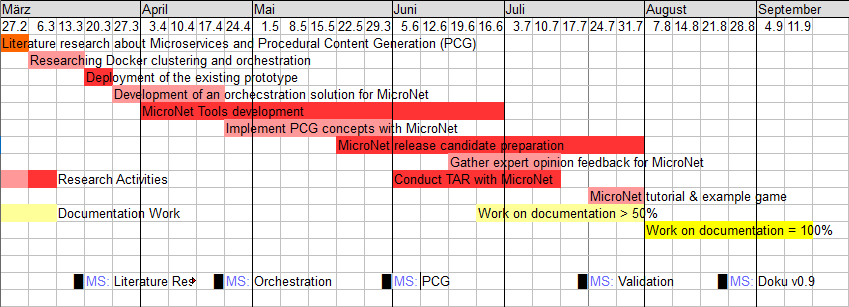
\includegraphics[width=1.2\textwidth]{images/ProjectPlan}
  	\caption{The project plan as defined at the beginning of this thesis.}
  	\label{fig:project_plan}
\end{figure}


\autoref{fig:project_plan} shows the project plan how it was established at the
beginning of this thesis. Unfortunately the project plan could not be fully met
and several activities were delayed.

Most noticeably \gls{pcg} was planned to be a prominent topic during this semester but
due to the workload introduced by composition and deployment topics the time
budget for \gls{pcg} shrank close to zero. This implies that the literature
about \gls{pcg} at the beginning of this thesis was a bit of a waste of time.

The work on the documentation also required a lot more effort than anticipated
because the documentation tended to grow quite rapidly. As a consequence all
other activities were suspended during July.

MicroNet Tools development was mostly on track but due to time consumption of
documentation work the final release of MicroNet and the associated
documentation were delayed until the end of August. Since the validation through
expert opinion relied on MicroNet being fully functional the validation survey
was executed much too late by the end of August when this thesis was almost
over.

All other activities were mainly on track and especially \gls{tar} was executed
just as planned in the middle of June.  
